
\subsection {Analyse du scénario}
Le projet doit donc être un système automatisé capable d'analyser des documents numérisés et d'en tirer des informations caractéristiques.
Ce logiciel doit ensuite se présenter sous la forme d'un moteur de recherche donnant la capacité à l'utilisateur de retrouver des documents de plusieurs façons différentes (mots clefs, ressemblance, ...).



\subsection {Scénario envisagé et retenu}
La Prefecture envisage donc la mise en place d'un système automatisant toute la chaine de travail, de la classification d'un document à sa recherche.
Afin de faciliter l'accès aux documents numérisés, la Prefecture désire aussi mettre en place un moteur de recherche afin de réduire le temps de recherche documentaire.

Le projet est donc séparé en deux blocs principaux :
Le classifier de documents et le moteur de recherche.

Le classifier doit être capable de lire n'importe quel document et d'en tirer des éléments caractéristiques internes, comme les parties prenantes, le type de document, la taxonomie, mais aussi les caractéristiques globales, comme par exemple décrire le document par un vecteur distinctif permettant de retrouver les documents similaires.
Toutes ces informations seront stockées dans des métadonnées associées à chaque documents.


Le moteur de recherche doit se baser sur les métadonnées crées par le classifier pour retrouver des documents.
On envisage des recherches par :
\begin {itemize}
\item taxonomie
\item similarité apparente
\item similarité de contenu
\item documents associés à une personne
\item documents associés à un document
\end {itemize}



\subsection {Critères de satisfaction}

 Les objectifs établis avec le commanditaire nous ont permis de séparer l'ensemble de ses exigences en deux parties :
\begin {itemize}
\item Exigences clés : Les objectifs qui impactent le cout et le développement du POC
\item Exigences critiques : Les objectifs qui sont essentiels et non négociables pour le POC
\end {itemize}

\par
Afin d'avoir un bon critère de satisfaction nous devons dans un premier temps répondre en priorité à l’ensembles des exigences critiques et d’y ajouter au plus les objectifs clés à notre POC. Au vu du temps et de la charge de travail, il est donc important de trouver ce bon compromis : 

\begin{figure}[h!]
	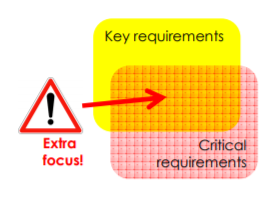
\includegraphics{images/requirements.png}
	\label{fig:MC}
\end{figure}		

	 Ci-dessous vous trouverez les exigences nécessaires pour répondre au mieux aux objectifs établie par le commanditaire :

Exigences clés :
\begin {itemize}
\item Permettre la recherche d’un document par similarité visuelle (pour
retrouver par exemple des permis de conduire, avec une couleur et un
format caractéristique)
\item Trouver les anciennes versions d’un document déjà stocké
\\
\end {itemize}

Exigences critiques :
\begin {itemize}
\item Être open source
\item Analyser le contenu sémantique d’un document
\item Classer les documents selon une taxonomie établie par la Préfecture
\item Permettre la recherche des documents associés à un document
\end {itemize}



